\documentclass{beamer}
\usepackage{setspace}
\usepackage{bm,color,float,epstopdf,amsthm,epstopdf}
\usepackage{multirow}
\title{Futures}
\newtheorem{result}{Result}
\renewcommand{\arraystretch}{2}
\begin{document}

\begin{frame}{Futures and Forwards}
\begin{itemize}
    \item Contract that requires future delivery of asset at agreed-upon price
    \item Long position: commit to purchase asset
    \item Short position: commit to deliver asset
    \item Forwards and futures do not have a premium
    \item Positions settled at maturity (no initial cash flow)
\end{itemize}
\end{frame}


\begin{frame}{Futures versus Forwards}
\begin{enumerate}
    \item Forwards
        \begin{itemize}
            \item Private contract between two parties 
            \item Not standardized
        \end{itemize}
    \item Futures \\
        \begin{itemize}
            \item Traded on an exchange
            \item Standardized contract 
        \end{itemize}
    \item Henceforth, I will refer to everything as a ``forward.''
\end{enumerate}
\end{frame}

\begin{frame}{Trading Strategies}
    \begin{itemize}
        \item Speculation
            \begin{itemize}
                \item Short if you believe price will fall
                \item Long if you believe price will rise
            \end{itemize}
        \item Hedging
            \begin{itemize}
                \item Long: Endowment fund will purchase stock in 3 months; manager buys forwards now to protect against rise in price
                \item Short: Hedge fund invests in long-term bonds; manager worries interest rates may increase and sells forwards
            \end{itemize}
    \end{itemize}
\end{frame}


\begin{frame}{Forwards Contracts}
\begin{itemize}
\item The trader in the long position is said to ``buy'' a contract; the short-side trader ``sells'' a contract. 
\item At maturity:
\begin{itemize}
\item Profit to long = Spot price at maturity - Original futures price
\item Profit to short = Original futures price - Spot price at maturity
\end{itemize}
\item The spot price is the actual market price of the commodity at the time of the delivery.
\end{itemize}
\end{frame}

\begin{frame}{Long and Short Forward}
    \begin{center}
        \begin{tabular}{cc}
            Long Forward: $S-K$ & Short Forward: $K-S$ \\
            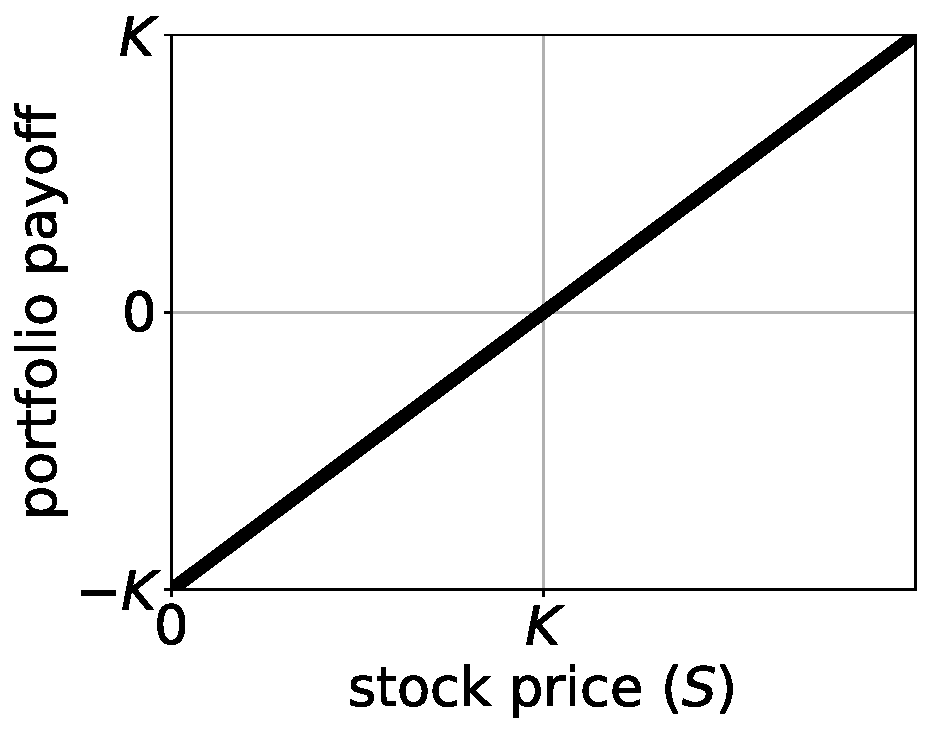
\includegraphics[scale=.3]{longforward} & 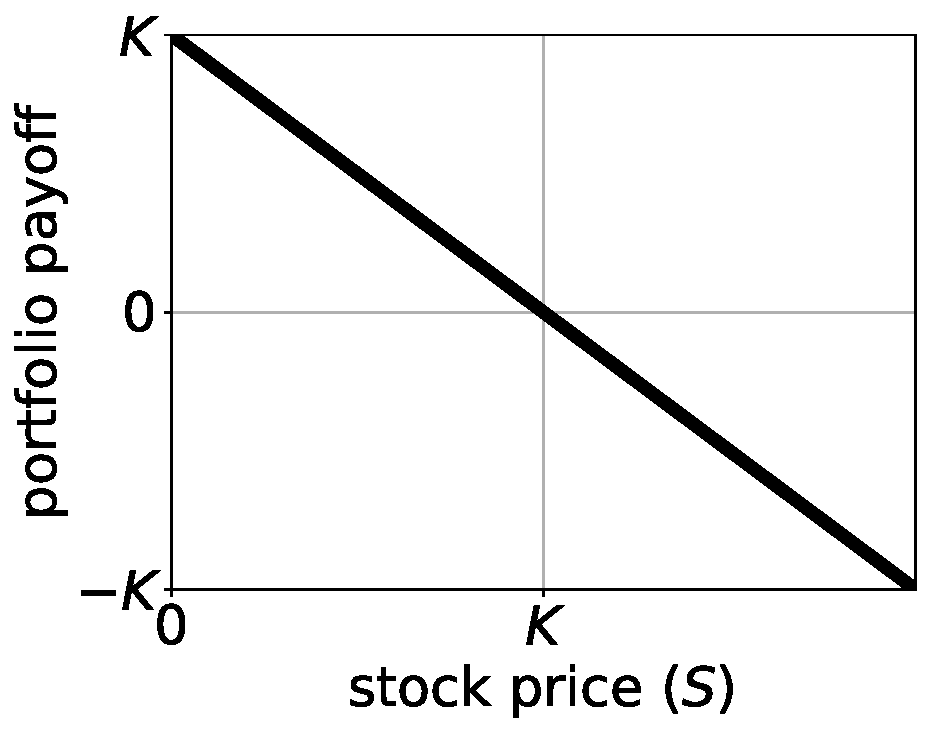
\includegraphics[scale=.3]{shortforward}
        \end{tabular}
    \end{center}
\end{frame}

\begin{frame}{Forward Payoff vs Call Payoff}
    \begin{center}
        \begin{tabular}{cc}
            Forward: $S-K$ & Call: $\max\{S-K,0\}$ \\
            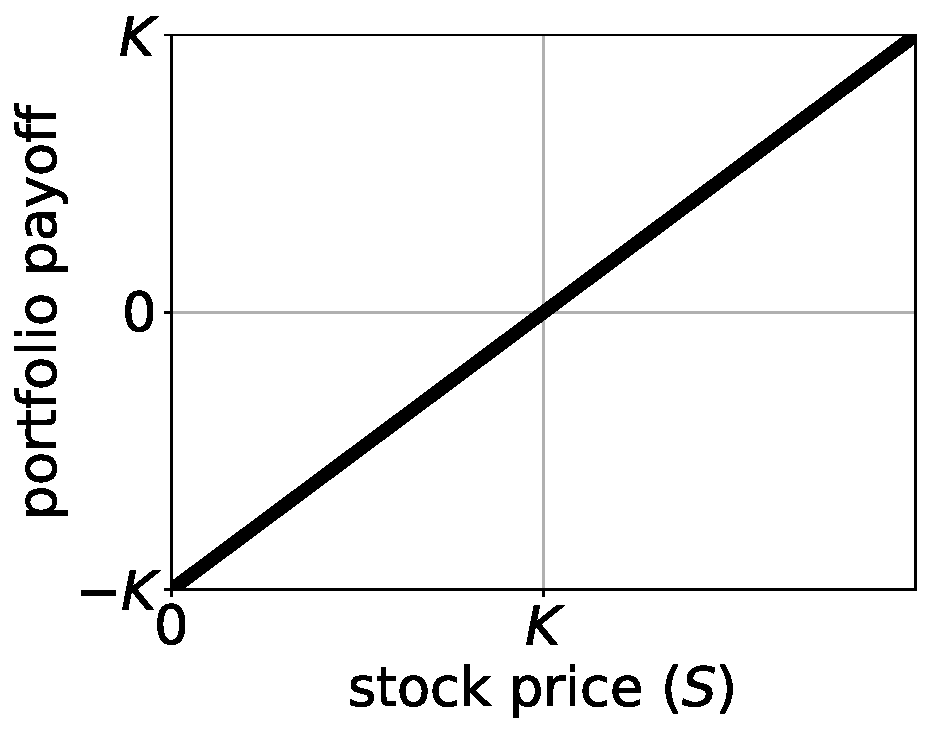
\includegraphics[scale=.3]{longforward} & 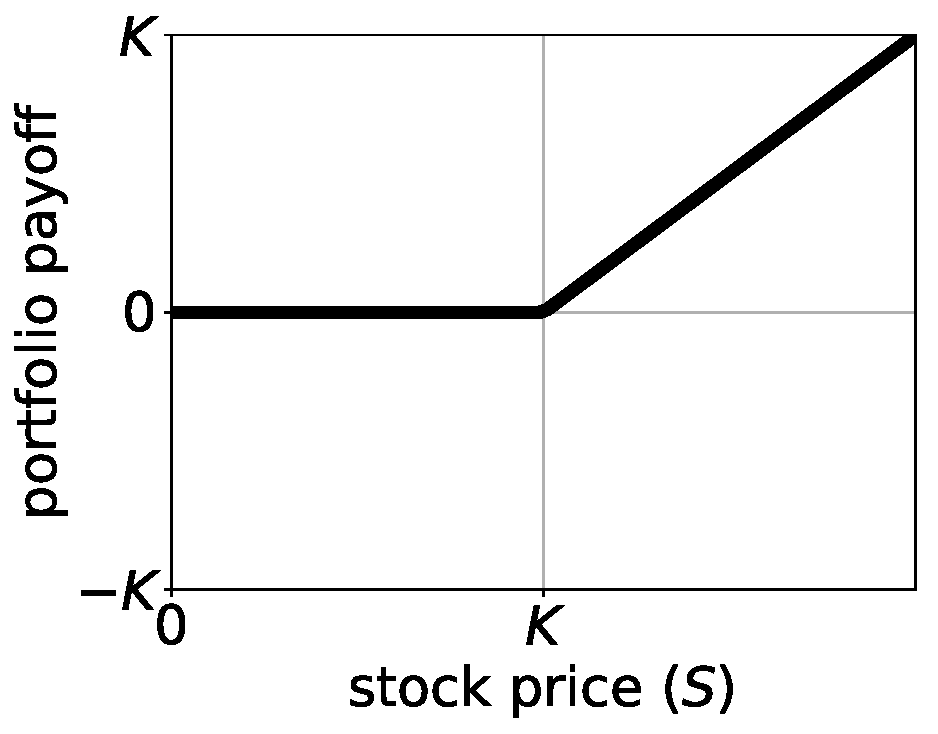
\includegraphics[scale=.3]{longcall}
        \end{tabular}
    \end{center}
\end{frame}


\begin{frame}{Basis and Hedging}
    \begin{itemize}
        \item Basis: difference between futures price and spot price $K-S_{t}$
        \item Spread Trade: take long position in forward with one maturity, short position in forward with another maturity.
    \end{itemize}
\end{frame}


\begin{frame}{Corporate Applications}
\begin{itemize}
\item Consider the case of an oil production company.  How much will the price of oil be in the future, when they are ready to sell the oil they produced?  The revenue of this company depends on oil prices, which are extremely volatile!
\item On the other hand, consider a company that has to buy oil as one of the inputs in the production process (airline company). This company has a problem that mirrors that of the oil production company. 
\item \textbf{Can forwards help these two firms?}
\end{itemize}
\end{frame}

\begin{frame}{Corporate Applications}
\begin{itemize}
\item \textbf{Yes!}  The two parties can enter into an agreement today that specifies the price at which the oil producer sells the oil to the other company in the future. 
\item Such an agreement will reduce the source of risk for both parties!  The oil producer delivers oil at a price agreed upon now, regardless of the market price at the time when oil is produced. 
\item This requires that BOTH parties be willing to lock in the price to be paid or received for delivery of the commodity. 
\item This can be achieved using forwards.
\end{itemize}
\end{frame}

\begin{frame}{Corporate Applications}
    \begin{center}
        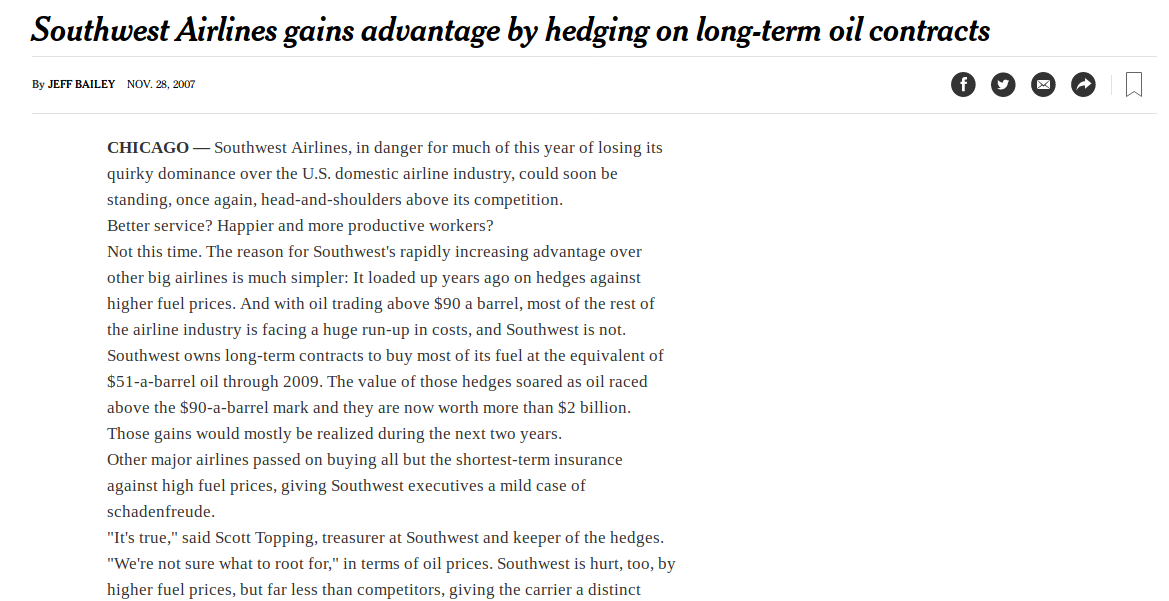
\includegraphics[scale=.3]{swa}
    \end{center}
\end{frame}

\begin{frame}{Types of Futures Contracts}
\begin{itemize}
\item Foreign Currencies
\item Agricultural Products
\item Metals and Energy
\item Interest Rate Futures
\item Equity Indexes
\end{itemize}
\end{frame}

\begin{frame}{Margin}
\begin{itemize}
\item In practice, traders may be required to post margin. 
\item Because \underline{both} parties to a futures contract are exposed to losses, \underline{both} must post margins. 
\end{itemize}
\end{frame}

\begin{frame}{Pricing}
\begin{itemize}
    \item Spot-Futures Parity-Theorem $K\overset{\text{``should''}}{=}S_{0}(1+r_{F})^{T}$
\end{itemize}
    \begin{center}
        \begin{tabular}{lccc}
            Security & Q & CF$_{0}$ & CF$_{T}$ \\ \hline
            Forward & 1 & 0 & $S_{T}-K$ \\ \hline\hline
            Stock & 1 & $-S_{0}$ & $S_{T}$ \\
            Risk-Free & $-K/(1+r)^{T}$ & $K/(1+r)^{T}$ & $-K$ \\ \hline
            & & $-S_{0}+K/(1+r)^{T}$ & $S_{T}-K$
        \end{tabular}
    \end{center}
\end{frame}

\begin{frame}{Board Problem 1}
    You're in sales at Goldman. A client wants a five-year forward on \$1m of the S\&P 500. The risk-free rate is 10\%. What should the price $K$ be? How do you hedge the position? What if the client tells you that he is willing to buy the forward for \$2m. What is your profit?  
\end{frame}

\begin{frame}{Board Problem 2}
Suppose that you buy a one-year forward on 10,000 shares of SPY, which currently sells for \$275. The risk-free rate is 10\%. You are required to post an initial margin of 20\% and meet a maintenance margin of 10\%
\begin{itemize}
    \item What should the forward price be? 
    \item How much margin (\$) must you post?  
    \item If SPY drops by 5\% tomorrow, what will the new forward price be?           
    \item How much margin (\%) do you have left? 
    \item Will you receive a margin call?  
    \item What is your return?
\end{itemize}
\end{frame}

\end{document}
